\documentclass{beamer}
\usepackage[utf8]{inputenc}
\usepackage[spanish]{babel}
\usetheme{metropolis}           % Use metropolis theme
\graphicspath{{images/}}

\usepackage{multicol}
\usepackage{listings}
\usepackage[default]{sourcesanspro}

\usepackage[scale=2]{ccicons}

\usepackage[
    type={CC},
    modifier={by-nc-sa},
    version={4.0},
]{doclicense}



\hypersetup{
    colorlinks=true,
    linkcolor=black,
    filecolor=magenta,
    urlcolor=cyan,
}

\title{Aprendizaje automático de un sistema interpretable de ayuda a la decisión para la estimación de la edad a partir de los huesos del pubis.}

\date{\today}
\author{\small Autor: Antonio David Villegas Yeguas \\ Directores: Óscar Cordón García y Sergio Damas Arroyo}
\institute[UGR]{Universidad de Granada\\
\medskip
\textit{advy99@correo.ugr.es}\\
\medskip
\url{https://github.com/advy99/TFG}
\doclicenseThis
}
\setbeamertemplate{caption}{\raggedright\insertcaption\par}

\begin{document}

 \maketitle

\begin{frame}{Índice}
\tableofcontents
\end{frame}




\section{Introducción y estado del arte del problema}
\begin{frame}{Estimación de la edad a partir de los huesos del pubis}

	\begin{columns}[T]
		\begin{column}{.5\textwidth}
			Problema complejo:
			\begin{itemize}
				\item No existe un método concreto.
				\item Trabajo subjetivo por parte de forenses.
				\item Falta de muestras para edades tempranas.
				\item Primera propuesta en 1920 por T. W. Todd \cite{todd}, clasificación en diez fases utilizando nueve características.
			\end{itemize}

		\end{column}

		\begin{column}{.5\textwidth}
			\begin{table}[H]
				\resizebox{\textwidth}{!}{%
					\begin{tabular}{|c|c|c|}
					\hline
					Crestas y surcos: Muy definidos & Superficie porosa irregular: Sí & Borde superior: Definido  \\ \hline
					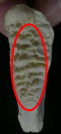
\includegraphics[scale = 0.75]{huesos/crestas_surcos_muy_definidos.png}  &   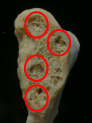
\includegraphics[scale = 0.75]{huesos/superficie_porosa_si.png} &  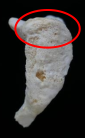
\includegraphics[scale = 0.75]{huesos/borde_superior_definido.png}  \\ \hline
					Nódulo óseo: Presente & Borde inferior: No definido & Borde dorsal: Definido \\ \hline
					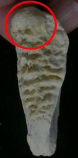
\includegraphics[scale = 0.75]{huesos/nodulo_oseo_presente.png} & 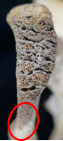
\includegraphics[scale = 0.75]{huesos/borde_inferior_no_definido.png} &  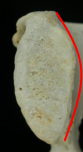
\includegraphics[scale = 0.75]{huesos/borde_dorsal_definido.png} \\ \hline
					Plataforma dorsal: Presente & Bisel ventral: En proceso de formación & Borde ventral: Muchas excrecencias \\ \hline
					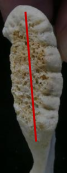
\includegraphics[scale = 0.75]{huesos/plataforma_dorsal_presente.png} & 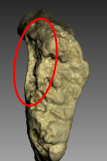
\includegraphics[scale = 0.75]{huesos/bisel_ventral_en_proceso_formacion.png} &   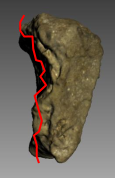
\includegraphics[scale = 0.75]{huesos/borde_ventral_muchas_excrecencias.png} \\ \hline
					\end{tabular}%
				}
				\caption{Algunos ejemplos de las características consideradas por Todd\cite{todd}.}\label{table:caracteristicas_todd}
			\end{table}
		\end{column}

	\end{columns}


\end{frame}

\begin{frame}[allowframebreaks]{Estado del arte}

\begin{itemize}
\item 1953 a 1973: Gilbert y McKern \cite{propuestaGilbert}. Cambio de enfoque a regresión, resultado expresado en un único valor y reducción de características.

\item 1990: J. M. Suchey y S. Brooks. Reducción del número de fases.

\item 2015: D. E. Slice y Algee-Hewitt. Escaneo de huesos utilizando Visión por Computador, clasificación con regresión lineal utilizando la propuesta de Suchey y Brooks. 41 muestras con una RECM de $17,15$ años.

\item 2015: D. Stoyanova, D. E. Slice y Algee-Hewitt. Modificación de las características utilizadas en su trabajo anterior. 57 muestras con una RECM de $19$ años.

\item 2018: A. Kotěrová, D. Navega, M. Štepanovský, Z. Buk, J. Brůžek y E. Cunha. Distintos modelos de aprendizaje, entre ellos regresión lineal, árboles de decisión y redes neuronales. 941 muestras, RECM de $12.1$ años y EAM de $9.7$ años.

\item 2021: J. C. Gámez-Granados, J. Irurita, R. Pérez, A. González, S. Damas, I. Alemán y O. Cordón (sometido a revista). Enfoque de Todd como un problema de clasificación ordinal, aprendizaje basado en reglas de forma iterativa. 892 muestras, RECM de $12,34$ años y 34 reglas fácilmente interpretables.

\end{itemize}

\end{frame}


\section{Objetivos}
\begin{frame}{Objetivos}
Nuestros objetivos serán:

\begin{enumerate}
	\item Obtener resultados sencillos, obtenidos a partir de modelos fácilmente interpretables.
	\item Tratar la alta dimensionalidad del problema.
	\item Estudiar el problema del número de muestras para resolver el problema.
\end{enumerate}

\end{frame}


\section{Inteligencia Artificial Explicable}
\begin{frame}{Inteligencia Artificial Explicable}


\end{frame}

\section{Propuesta e implementación}
\begin{frame}{Conjunto de datos}


\end{frame}

\begin{frame}{Algoritmos}


\end{frame}

\begin{frame}{Tecnologías utilizadas}


\end{frame}

\section{Análisis de resultados y comparación con el estado del arte}
\begin{frame}{Resultados}


\end{frame}

\begin{frame}{Importancia del sobremuestreo}


\end{frame}

\begin{frame}{Mejores expresiones obtenidas}


\end{frame}

\begin{frame}{Comparación con el estado del arte}


\end{frame}



\section{Conclusiones}
\begin{frame}{Conclusiones}


\end{frame}

\section{Bibliografía}
\begin{frame}[allowframebreaks]{Bibliografía}

\begin{thebibliography}{9}

	\bibitem{todd}

	\href{https://onlinelibrary.wiley.com/doi/abs/10.1002/ajpa.1330030301}{\scriptsize T. W. Todd, “Age changes in the pubic bone,” American Journal of Physical Anthropology, vol. 3, no. 3, pp. 285–328, 1920.}

	\bibitem{propuestaGilbert}

	\href{https://onlinelibrary.wiley.com/doi/abs/10.1002/ajpa.1330380109}{Gilbert, B. M., \& McKern, T. W. (1973). A method for aging the female os pubis. American Journal of Physical Anthropology, 38(1), 31-38.}

\end{thebibliography}


\end{frame}


\section{Preguntas}


\end{document}
